% \PassOptionsToPackage{darkblue}{xcolor}
\documentclass[10pt,aspectratio=169]{beamer}
% \usecolortheme{dove}
% \usetheme{Goettingen}

\usecolortheme{seagull}

\usepackage[
    autocite=superscript,
    backend=biber,
    style=authoryear-comp
    ]{biblatex}
\DeclareCiteCommand{\supercite}[\mkbibsuperscript]
  {\iffieldundef{prenote}
     {}
     {\BibliographyWarning{Ignoring prenote argument}}%
   \iffieldundef{postnote}
     {}
     {\BibliographyWarning{Ignoring postnote argument}}}
  {\usebibmacro{citeindex}%
   \bibopenbracket\usebibmacro{cite}\bibclosebracket}
  {\supercitedelim}
  {}

\addbibresource{bibliography.bib}
% New notation ------------------------------------------------------------------
\newcommand{\expo}{E}
\newcommand{\Expo}{\mathbf{\expo{}}}
\newcommand{\expod}[1]{\expo_{#1}^D}
\newcommand{\expoc}[1]{\expo_{#1}^C}
\newcommand{\expoi}[1]{\expo_{#1}^I}

\newcommand{\covar}{\mathbf{x}}
\newcommand{\Covar}{\mathbf{X}}
\newcommand{\latent}{\mathbf{z}}
\newcommand{\Latent}{\mathbf{z}}

\newcommand{\Event}{\mbox{P}}
\newcommand{\pset}[1]{\mathcal{P}\left(#1\right)}
\newcommand{\size}[1]{\left|#1\right|}

%\newcommand{\logit}[1]{\mbox{logit}^{-1}\left(#1\right)}
% -------------------------------------------------------------------------------

% -------------------------------------------------------------------------------

\usepackage{booktabs,tabularx}
\usepackage{fancybox}
\usepackage{ulem}
% Mathematical functions
% DELETED!
\renewcommand{\Pr}[1]{{\mathbb{P}\left(#1\right) }}
% DELETED!
% DELETED!
% DELETED!
% DELETED!
% DELETED!

% DELETED!
\newcommand{\sufstats}[1]{s\left(#1\right)}
\renewcommand{\exp}[1]{\mbox{exp}\left\{#1\right\}}
\renewcommand{\log}[1]{\mbox{log}\left\{#1\right\}}
\newcommand{\transpose}[1]{{#1}^\mathbf{t}}
\renewcommand{\t}[1]{\transpose{#1}}

\newcommand{\s}[1]{\sufstats{#1}}
\newcommand{\SUFF}{\mathcal{S}}
\newcommand{\Suff}{\mathbf{S}}
\newcommand{\suff}{\mathbf{s}}

\renewcommand{\beta}{\theta}
\newcommand{\weight}{\mathbf{w}}
\newcommand{\Weight}{\mathbf{W}}

% Objects
% DELETED!
% DELETED!
\newcommand{\Graph}{\mathbf{G}}
\newcommand{\graph}{\mathbf{g}}
\newcommand{\GRAPH}{\mathcal{G}}
\newcommand{\Adjmat}{Y}
\newcommand{\adjmat}{y}
\newcommand{\ADJMAT}{\mathcal{Y}}

\newcommand{\INDEPVAR}{\mathcal{X}}
\newcommand{\Indepvar}{X}
\newcommand{\indepvar}{x}

\newcommand{\normconst}{\kappa\left(\params, \Indepvar\right)}

\graphicspath{{./figures/}{.}{./terms/}}


%% NEED THIS FOR CANCY TEX
\usepackage{pstricks}

% Colors
\definecolor{USCCardinal}{HTML}{990000} % 153 0 0 in RGB
\definecolor{USCGold}{HTML}{FFCC00}
\definecolor{USCGray}{HTML}{CCCCCC}

% \bibliography{bibliography.bib}

\def\ergmito{ERGM\textit{ito}}
\def\ergmitos{\ergmito{}\textit{s}}
% Mathematical functions
\newcommand{\isone}[1]{{\boldsymbol{1}\left( #1 \right)}}
\renewcommand{\Pr}[1]{{\mathbb{P}\left(#1\right) }}
\newcommand{\f}[1]{{f\left(#1\right) }}
\newcommand{\Prcond}[2]{{\mathbb{P}\left(#1\vphantom{#2}\;\right|\left.\vphantom{#1}#2\right)}}
\newcommand{\fcond}[2]{{f\left(#1|#2\right) }}
\newcommand{\Expected}[1]{{\mathbb{E}\left\{#1\right\}}}
\newcommand{\ExpectedCond}[2]{{\mathbb{E}\left\{#1\vphantom{#2}\right|\left.\vphantom{#1}#2\right\}}}
\renewcommand{\exp}[1]{\mbox{exp}\left\{#1\right\}}

\newcommand{\Likelihood}[2]{\text{L}\left(#1 \left|\vphantom{#1}#2\right.\right)}

\newcommand{\loglik}[1]{\mathcal{L}\left(#1\right)}
\newcommand{\logit}[1]{\mbox{logit}\left(#1\right)}


% Mathematical Annotation -------------------------------
% Modify this so that it matches the P01 convention overall

% Tree
\newcommand{\phylo}{\Lambda{}} % The actual tree
\newcommand{\aphylo}{D{}}      % The annotated phylogenetic tree
\newcommand{\aphyloObs}{\tilde \aphylo{}} % The observed annotated phylogenetic tree
\newcommand{\parent}[1]{\mathbf{p}\left(#1\right)}
\newcommand{\offspring}[1]{\mathbf{O}\left(#1\right)}
\newcommand{\nodes}{\mathcal{N}{}}
\newcommand{\edges}{\mathcal{E}{}}

\newcommand{\class}[1]{C_{#1}{}}

% Annotations
\newcommand{\ANN}{\mathbf{Y}{}} % Matrix of "real" annotations
\newcommand{\Ann}{\mathbf{y}{}}
\newcommand{\ann}[1]{y_{#1}} % single element of "real" annotations
\newcommand{\constraints}{\mathcal{C}{}} % Taxon constraints

% Obs Annotations
\newcommand{\ANNOBS}{\mathbf{Y}^{obs}}%{Z{}} \mathbf{X}^{obs}{}
\newcommand{\AnnObs}{\mathbf{y}^{obs}}
\newcommand{\annObs}[1]{y_{#1}^{obs}}%{z{}}  x_{#1}^{obs

% Pred. Annotations
\newcommand{\AnnPred}{\hat \Ann{}}
\newcommand{\annPred}[1]{\hat {\ann{#1}}}

% Type o event
\newcommand{\type}{T}

% Leaf nodes
\newcommand{\Leaf}{L{}}

% Shortest path
\newcommand{\Geodesic}{\text{T}{}}
\newcommand{\geodesic}{\tau{}}

\newcommand{\Params}{\Omega{}}
\newcommand{\params}{\omega{}}

% Parameters
\newcommand{\gain}{\mu_{01}{}}
\newcommand{\loss}{\mu_{10}{}}
\newcommand{\misszero}{\psi_{01}{}}
\newcommand{\missone}{\psi_{10}{}}
\newcommand{\proot}{\pi}


% Change statistic
\newcommand{\chng}[1]{\delta\left(\ann{#1}:0\to1\right)}

\newcommand{\pgraph}{\Ann}
\newcommand{\snamed}[2]{\s{#1}_{\mbox{#2}}}

% For the revision
\usepackage{marginnote}
\newcommand{\revtext}[2]{\textcolor{black}{#2}\marginnote{#1}}

% Features
\newcommand{\Features}{X{}}
\newcommand{\features}[1]{x{#1}}

%%%%%%%%%%%%%%%%%%%%%%%%%%%%%%%%%%%%%%%%%
% These lines should usually go into a .sty file,
% but I'll leave them here so that it's easier to
% see how to customise a Beamer theme.
% Remember, the Beamer manual is your friend!!
% http://texdoc.net/pkg/beamer
%
%% So if your re-definitions have a @ somewhere, you
%% _MUST_ put a \makeatletter before these lines and then
%% \makeatother after them. This trick can only be done
%% in the preamble! BUT if you're doing these re-definitions
%% in a .sty file (so that you \usepackage it later), you
%% don't need the \makeatletter and \makeatother.
\makeatletter

%% Set the left and right margins
\setbeamersize{text margin left=1em,text margin right=1em}

%% FONTS
\setbeamerfont{title}{series=\bfseries,size=\LARGE}
\setbeamerfont{subtitle}{series=\bfseries,size=\Large}
\setbeamerfont{frametitle}{series=\bfseries,size=\small}
\setbeamerfont{block title}{series=\bfseries,size=\normalsize}
\setbeamerfont{footline}{size=\normalsize}

%% COLOURS
%% If you'd like everything to have the same colour
\usebeamercolor{structure}
\setbeamercolor{normal text}{fg=structure.fg}

%% Add a line after the frametitle
\addtobeamertemplate{frametitle}{}{\vspace*{-1ex}\rule{\textwidth}{1pt}}

%% Use circular discs as itemized list markers;
%% there's an existing option in Beamer for it so I'll use it
\setbeamertemplate{itemize items}[circle]

%% Remove default navigation symbols (We'll add the ones we need in the footline
\setbeamertemplate{navigation symbols}{}


%% And before the footline... actually we'd like to re-define
%% the footline
\setbeamertemplate{footline}{%
	%% Beamer headlines and footlines are always full-paperwidth, so if you want the horizontal line to
	%% not span it entirely you'll need to do a bit of arithmetic
	\centering
	\begin{minipage}{\dimexpr\paperwidth-\beamer@leftmargin-\beamer@rightmargin\relax}
		\centering
		\rule{\linewidth}{1pt}\vskip2pt
		\usebeamerfont{footline}%
		\usebeamercolor{footline}%
		%% The frame number smack in the middle
		\hfill\insertpagenumber/\inserttotalframenumber
		\hfill%
		%% ONLY the navigation symbols we want at the far right.
		%% We use an \llap so that it takes up zero width, and doesn't throw the page number off-centre!
		\llap{\insertframenavigationsymbol\insertbackfindforwardnavigationsymbol}\par
	\end{minipage}\vskip2pt
}

\makeatother
%%%% END STYLE CUSTOMISATION %%%%%%%%%%%%

% Slide numbers
\newcounter{frame}[frame]
\setbeamertemplate{footline}[frame number] 

\graphicspath{{.}{fig/}}

\title[Predicting Gene Functions with Mech. ML]{Predicting of Gene Functions by Leveraging Biological Insights with Mechanistic Machine Learning\\\includegraphics[width=.2\linewidth]{DALL·E 2022-12-07 21.41.30}\vspace{-.5cm}}
\author[\hyperlink{https://ggv.cl}{https://ggv.cl}]{George G. Vega Yon, Ph.D.\\{\small \color{darkgray}george.vegayon@utah.edu}\vspace{-.5cm}}
\institute[UofUEpi]{Division of Epidemiology @ University of Utah}
\date{May 3rd, 2023 @ USC IMAGE\vspace{-.5cm}}

%%%%%%%%%%%%%%%%%%%%%%%%%%%%%%%%%%%%%%%%%%%%%%%%%%%%%%%%%%%%%%%%%%
%%%%%%%%%%%%%%%%%%%%%%%%%%%%%%%%%%%%%%%%%%%%%%%%%%%%%%%%%%%%%%%%%%
\newcommand{\toc}[0]{\begin{frame}{Table of Contents}
    \tableofcontents[current]
\end{frame}}

\newcommand{\tocsub}[0]{\begin{frame}{Table of Contents}
    \tableofcontents[currentsubsection]
\end{frame}}

\newcommand{\byside}[3]{\begin{minipage}[t]{#1\linewidth}%
		\bigskip
		\centering%
		\shadowbox{\Large #2}\hfill\\\bigskip%
		#3%
\end{minipage}}

%%%%%%%%%%%%%%%%%%%%%%%%%%%%%%%%%%%%%%%%%%%%%%%%%%%%%%%%%%%%%%%%%%
%%%%%%%%%%%%%%%%%%%%%%%%%%%%%%%%%%%%%%%%%%%%%%%%%%%%%%%%%%%%%%%%%%
\begin{document}

\begin{frame}
    \maketitle
    {\scriptsize Collaborators: Paul Thomas, Paul Marjoram, Huaiyu Mi, Christopher Williams (USC), Alun Thomas (UofU)}
\end{frame}

\begin{frame}{Table of Contents}
    \tableofcontents
    You can download the slides from \url{https://ggv.cl/image2023}
\end{frame}

%%%%%%%%%%%%%%%%%%%%%%%%%%%%%%%%%%%%%%%%%%%%%%%%%%%%%%%%%%%%%%%%%%
%%%%%%%%%%%%%%%%%%%%%%%%%%%%%%%%%%%%%%%%%%%%%%%%%%%%%%%%%%%%%%%%%%
\section{Preliminaries}\toc{}

\begin{frame}<123123>
	\frametitle{Gene Function}
	
	Encode the synthesis of genetic products that ultimately are related to a
	particular aspect of life, for example
	
	\def\tmpwidth{.9\linewidth}
	
	\begin{table}
		\begin{tabular}{*{3}{m{.31\linewidth}<{\centering}}}
			\onslide<2->\bf Molecular function & %
			\onslide<3->\bf Cellular component & %
			\onslide<4->\bf Biological process \\
			\onslide<2->\href{http://amigo.geneontology.org/amigo/term/GO:0005215}{Active transport GO:0005215}& %
			\onslide<3->\href{http://amigo.geneontology.org/amigo/term/GO:0004016}{Mitochondria GO:0004016} & %
			\onslide<4->\href{http://amigo.geneontology.org/amigo/term/GO:0060047}{Heart contraction GO:0060047} \\
			\onslide<2->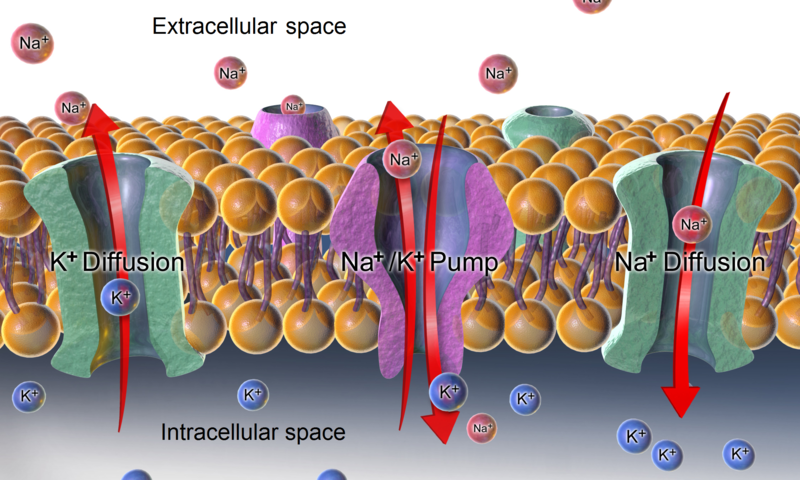
\includegraphics[width=\tmpwidth]{Sodium-potassium_pump_and_diffusion.png} & %
			\onslide<3->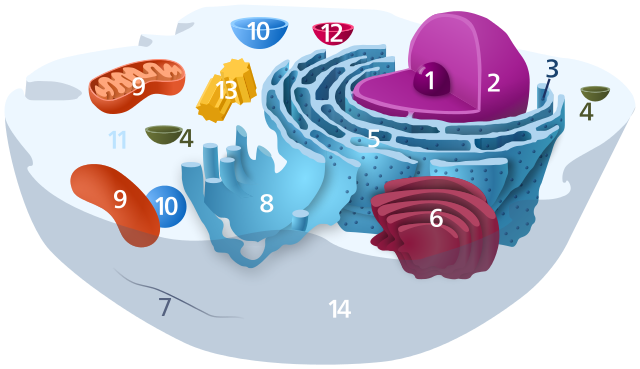
\includegraphics[width=\tmpwidth]{640px-Animal_Cell-svg.png} & % 
			\onslide<4->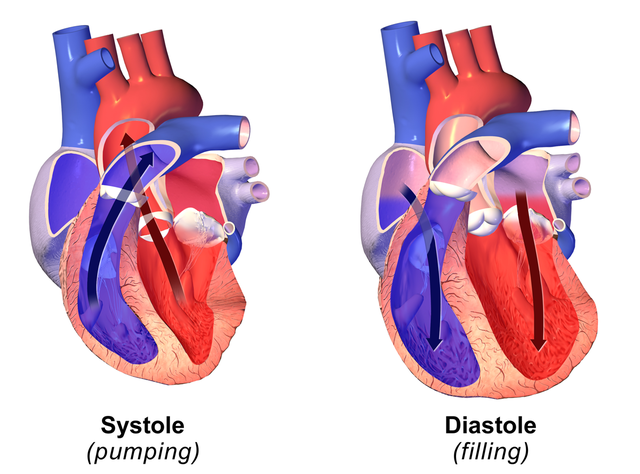
\includegraphics[width=\tmpwidth]{Systolevs_Diastole.png}
		\end{tabular}
	\end{table}
	
\end{frame}

\begin{frame}<123123>{Gene Function: the Gene Ontology Project}
    \begin{figure}

\includegraphics[width=.4\linewidth]{fig/go-logo.png}
\end{figure}

\begin{itemize}[<+->]
\item The GO project has $\sim$ 43,000 validated terms, $\sim$ 7.4M annotations on $\sim$ 5,200 species.
\item About $\sim$ 700,000 annotations are on human genes.
\item Only half of the human gene annotations are based on experimental evidence.
% \item Roughly half of human genes ($\sim$ 10,000 / 20,000) have some
% form of annotation.
% \item We know something of less than 10\% of known genes (near 1.7M).
\item About $\sim$ 173,000 publications have used the GO.% 40610
%\item An important effort of the GO has to do with phylogenetics...
\end{itemize}

\vfill
\hfill \small \textbf{source}: Statistics from \url{http://pantherdb.org/panther/summaryStats.jsp} and \url{http://geneontology.org/stats.html}\normalsize

\end{frame}

\begin{frame}{Predicting Gene Function: State-of-the-art}
	
	Sequences, phylogenomics, and ML.
	
	\begin{itemize}[<+->]
		\item \textbf{BLAST}\autocite{altschulBasicLocalAlignment1990}: Prediction by sequence homology ($\sim$ 105,000 citations).
		\item \textbf{SIFTER}\autocite{Engelhardt2005, Engelhardt2011}: An evolutionary model of gene function/loss using phylogenetics.
		\item \textbf{aphylo}\autocite{VegaYon2021} (by yours truly): Another phylo-based method. Leverages negative annotations and pooled trees.
		\item \textbf{Phylo-PFP}\autocite{Jain2019}: A BLAST-based adding phylogenetic based distances.
		\item \textbf{DeepGOPlus}\autocite{kulmanovDeepGOPlusImprovedProtein2019}: One of the top-performing models in the literature, uses a 2D convolutional neural network on gene sequences.
		%		\begin{itemize}
			%			\item At most, three hidden layers (tried others)
			%			\item Typical activations relu and sigmoid
			%			\item Focus on feature engineering
			%			\item Beyond sequence similarity, there is \textbf{no biological theory supporting the model}.
			%		\end{itemize}
		\item \textbf{GOLabeler}\autocite{youGOLabelerImprovingSequencebased2018}: Top performing tool according to the \textit{Critical Assessment of Function Annotation} [CAFA] challenge\autocite{Zhou2019cafa}, is an ensemble of various simple ML methods, including K-means and logistic regression.
            \item \textbf{DeepFRI}\autocite{gligorijevicStructurebasedProteinFunction2021}: Uses Graph Convolutional Neural Networks (GCNs) to predict function based on protein structure and genetic sequence.
	\end{itemize}

%	\vfill \uncover<9->{None of the ML-based methods relies on biological theory (mechanistic models).}
	\vfil \uncover<8->{In the latest CAFA, \textbf{none}  of the top-performing methods scored an AUC above 0.60, and most were outperformed by BLAST\autocite{Zhou2019}, which annotates using homology based on sequence similarity.}	
\end{frame}



\section{Evolution of Gene Function}
\toc{}

% \begin{frame}[c]
% %	\frametitle{Uncovering the role of genes}
	
% 	\Large Is gene \textit{XYZ} involved in process \textit{ABC}?\normalsize\bigskip
	
% 	\begin{minipage}[t]{.33\linewidth}
% 		\centering
% 		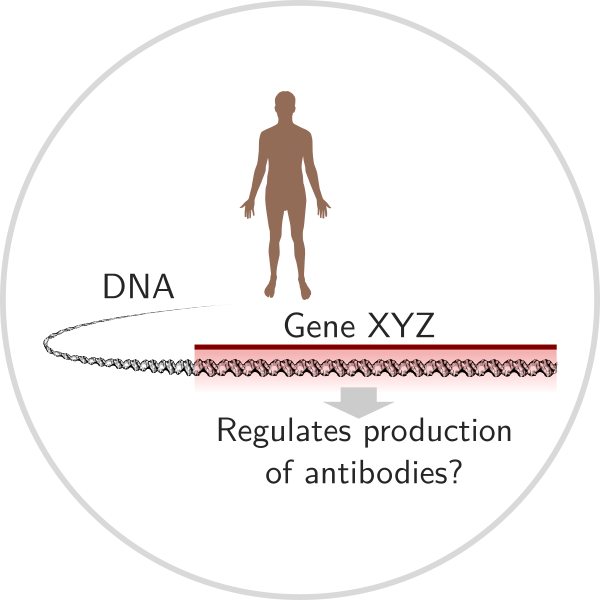
\includegraphics[width=1\linewidth]{aphylo-data-0.png} \\
% 		Complex to directly assess
% 	\end{minipage}\hfill
% 	\uncover<2->{\begin{minipage}[t]{.33\linewidth}
% 		\centering
% 		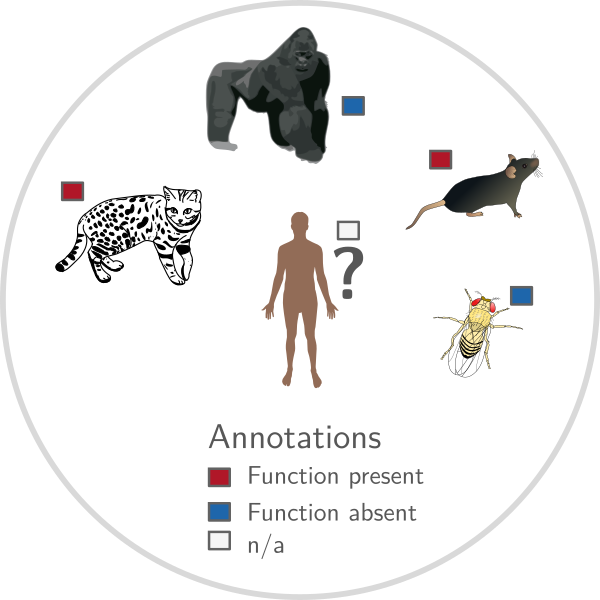
\includegraphics[width=1\linewidth]{aphylo-data-1.png}\\
% 		But we may know from other species
% 	\end{minipage}}\hfill
% 	\uncover<3->{\begin{minipage}[t]{.33\linewidth}
% 		\centering
% 		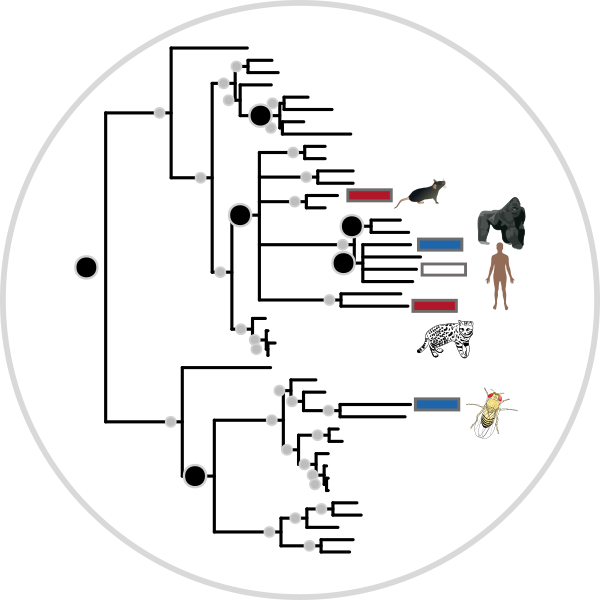
\includegraphics[width=1\linewidth]{aphylo-data-2.png}\\
% 		And we further know how these are \textit{evolutionary} connected
% 	\end{minipage}}\hfill
	
% % \bigskip\uncover<4>{\raggedleft\Large ... let's rephrase the question. \normalsize}

% \end{frame}

\begin{frame}[c,label=aphylo-prob-diagram]{Our progress so far...}
\begin{center}
    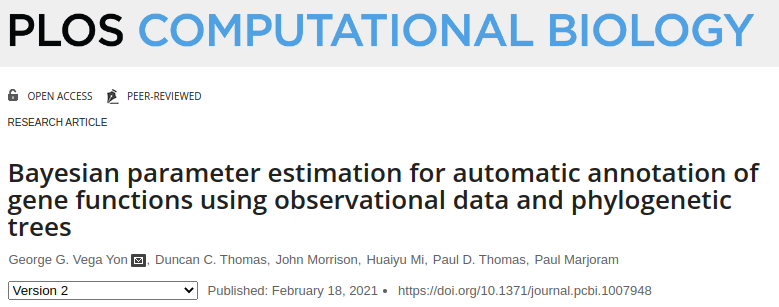
\includegraphics[width=.6\linewidth]{fig/aphylo-plos-comp-bio.png}
\vfill
    \normalsize Is the human gene \textbf{XYZ} involved in process \textbf{ABC}, \uline{given what we know about that for other \textit{related} species}?
\vfill
    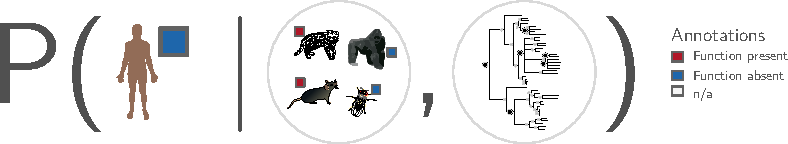
\includegraphics[width=.8\linewidth, clip, trim={0 0 0 0}]{aphylo-data-probability.pdf}
\end{center}
\end{frame}

\begin{frame}{Evolution of Gene function (of one function)}

Built a big model (lots of trees and annotations) called aphylo:

\begin{center}
\begin{minipage}{.44\linewidth}
    \begin{itemize}[<+->]
        \item Only two sources of data: Phylogenetic tree (\url{pantherdb.org}) and functional annotations (\url{geneontology.org}).
        \item Leverage negative annotation of GO terms (NOT).
        \item Use Felsenstein's tree pruning algorithm to compute tree likelihood.
        \item Fit pooled models featuring thousands of annotations in hundreds of trees (with split-second prediction capability).
    \end{itemize}
\end{minipage}
\begin{minipage}{.55\linewidth}
    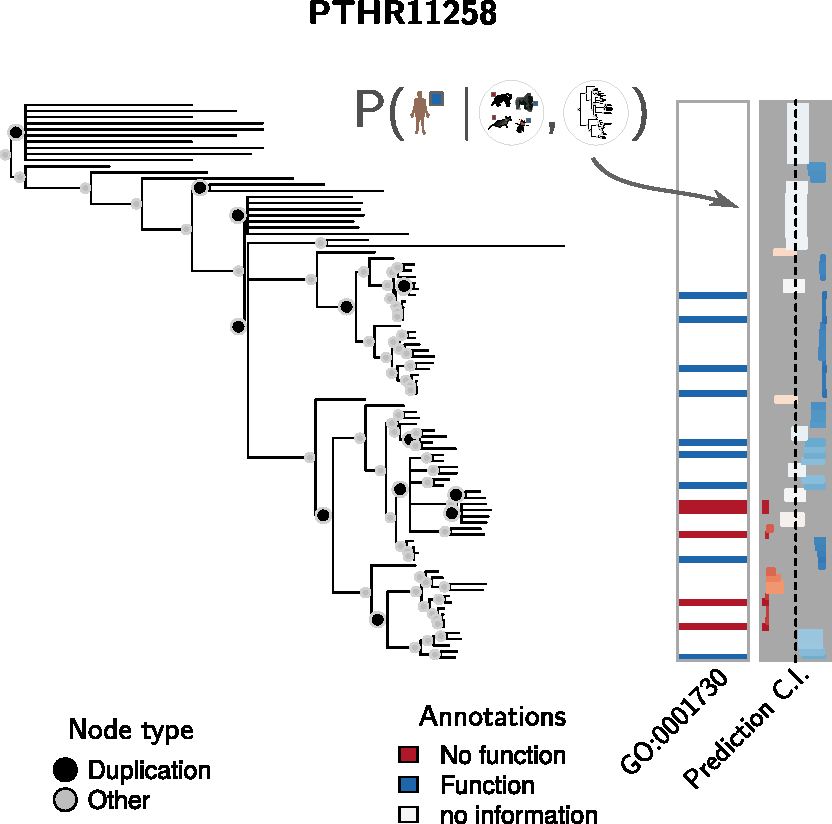
\includegraphics[width=.8\linewidth, clip, trim={0 0 0 1.5cm}]{example-trees-good1-parts-1b.pdf}
\end{minipage}
\end{center}

\vfil\hfill\uncover<4->{... But what if we wanted to deal with multiple functions?}
  
\end{frame}

\begin{frame}{Evolution of Gene function (multiple functions)}
Tapping into Evol. Theory (part of Proj. 3)\\\bigskip

\begin{center}
\begin{minipage}{.44\linewidth}
\begin{itemize}[<+->]
    \item A fundamental part of Fun. Evol. is Duplication Events.
    \item Furthermore, knowing what happened to gene A (\textit{e.g.}, neofunctionalization) is highly informative to learn about the functional state of B.
    \item One way to model this is using a Markov Transition Model (as in SIFTER).
\end{itemize}
\end{minipage}
\begin{minipage}{.55\linewidth}
    \begin{figure}
    \centering
    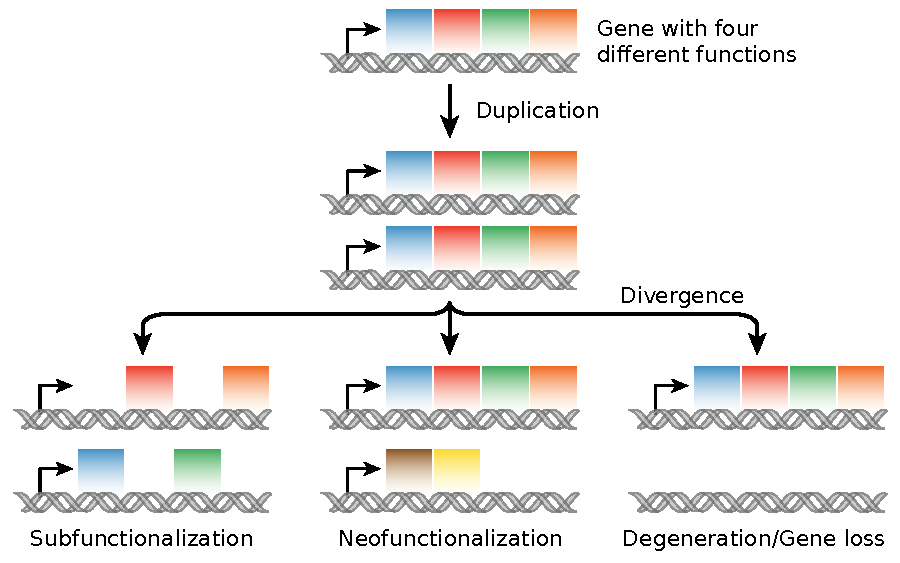
\includegraphics[width=1\linewidth]{fig/Evolution_fate_duplicate_genes_-_vector.pdf}
    \caption{A key part of molecular innovation, gene duplication provides an opportunity for new functions to emerge (\href{https://en.wikipedia.org/wiki/File:Evolution_fate_duplicate_genes_-_vector.svg}{wikimedia})}
    \label{fig:duplication}
    \end{figure}
\end{minipage}
\end{center}

\end{frame}



% ------------------------------------------------------------------------------
\begin{frame}[c]{Evolution of Gene function (multiple functions) (cont.)}
	
	If we wanted to build a model with 3 functions, we would need to estimate...\\\bigskip
	
	\begin{minipage}[t]{.40\linewidth}
		\centering
		\shadowbox{Full Markov Transition Matrix}\\\bigskip
		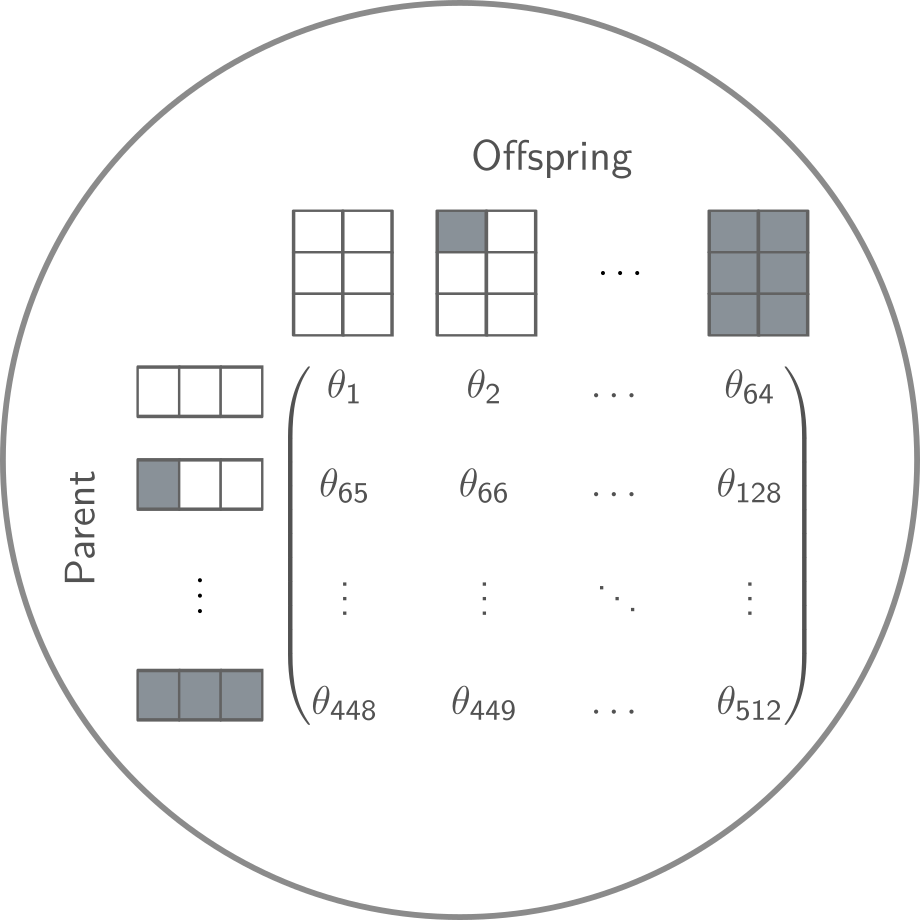
\includegraphics[width=.8\linewidth]{aphylo-ergm-eq1.png} \\
			\vfill 512 parameters
	\end{minipage}\hfill
	\begin{minipage}[t]{.19\linewidth}
		\centering 
		\uncover<3->{
			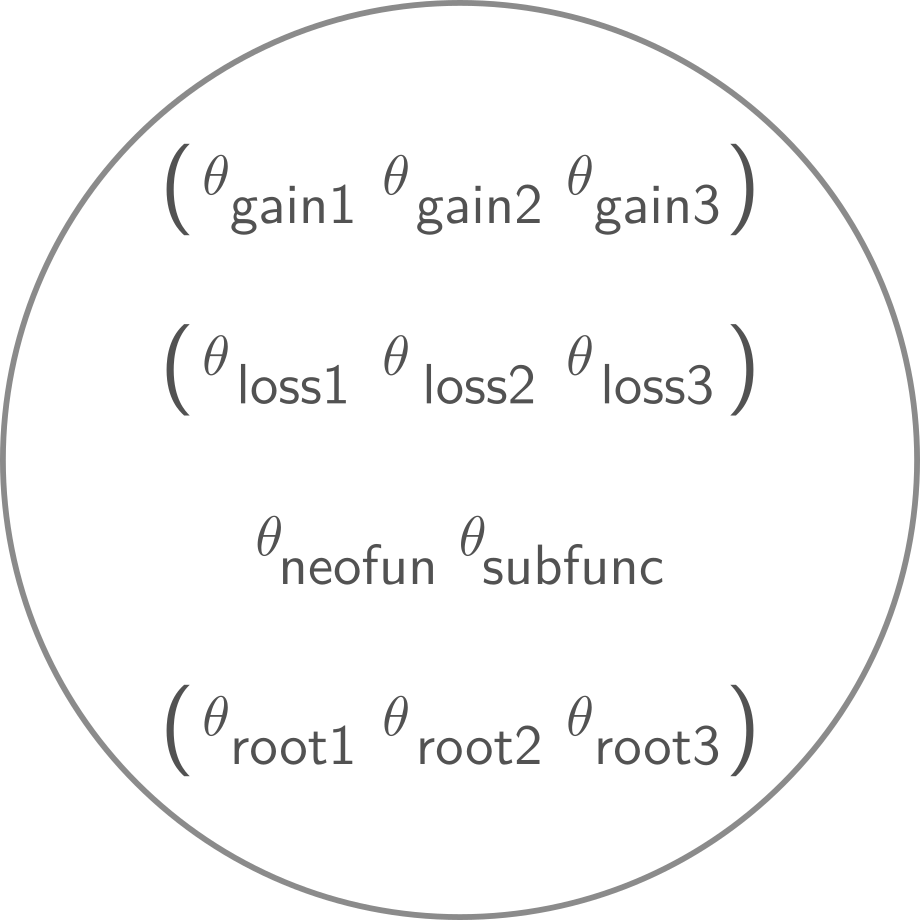
\includegraphics[width=.8\linewidth]{aphylo-ergm-eq2.png}\\
			Easier to fit \\
			Easier to interpret}	
	\end{minipage}\hfill
	\uncover<2->{\begin{minipage}[t]{.40\linewidth}		
		\centering
		\shadowbox{Sufficient statistics}\\\bigskip
		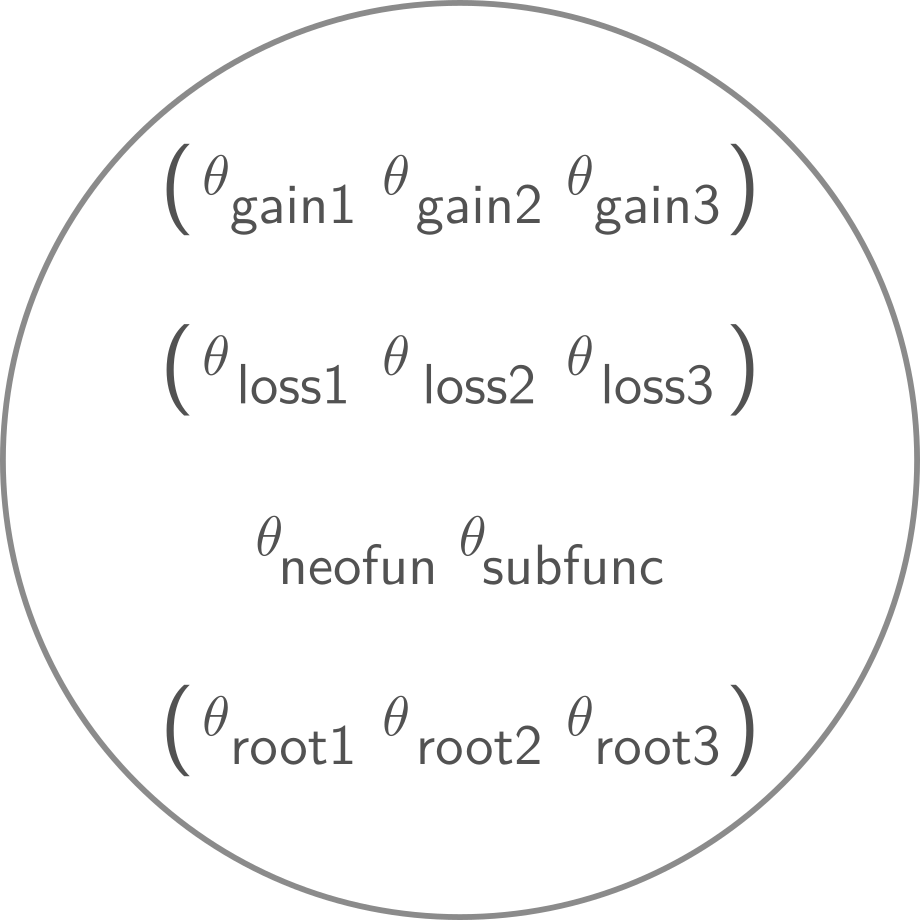
\includegraphics[width=.8\linewidth]{aphylo-ergm-eq2.png} \\
			\vfill 11 parameters (for example)
	\end{minipage}}
\end{frame}



\begin{frame}
\begin{minipage}[t]{.02\linewidth}\hspace{-1cm}
	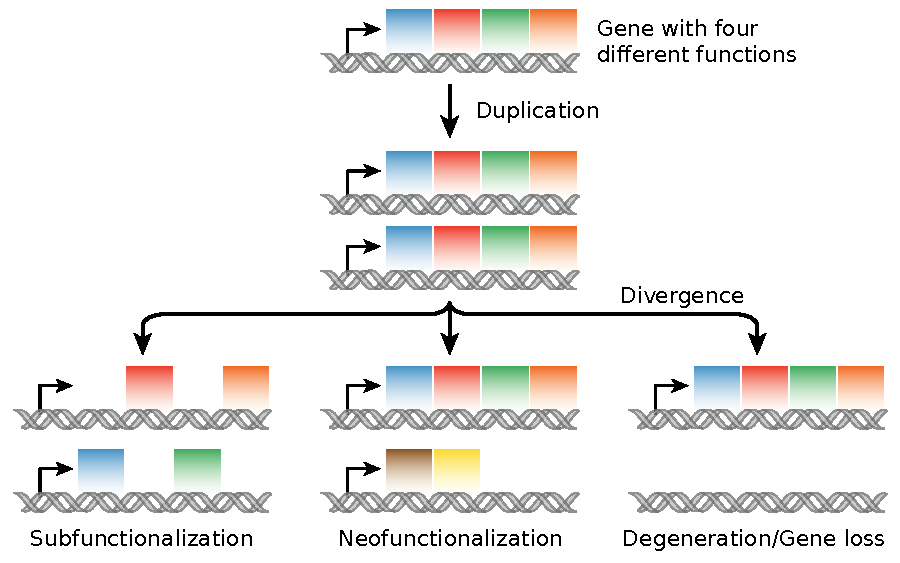
\includegraphics[width=6\linewidth]{fig/Evolution_fate_duplicate_genes_-_vector.pdf}\vspace{-3cm}
\end{minipage}

\vfill

\begin{minipage}[b]{.95\linewidth}
\footnotesize
	\def\fwidth{.55\linewidth}
	\begin{table}
	\begin{tabular}{m{.14\linewidth}<\centering m{.25\linewidth}m{.46\linewidth}}
	\toprule
	Rep. & Description & Definition  \\ \midrule
	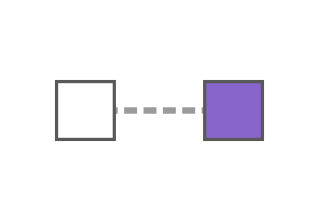
\includegraphics[width=\fwidth]{fig/term-gain.png} & %
		Gain of function & $(1 - x_p)\sum_{n:n\in Off}x_n$  \\
	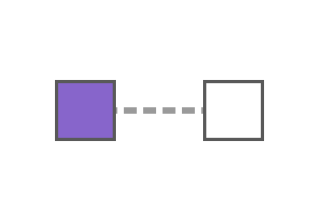
\includegraphics[width=\fwidth]{fig/term-loss.png} & %
		Loss of function & $x_p\sum_{n:n\in Off}(1 - x_n)$  \\
	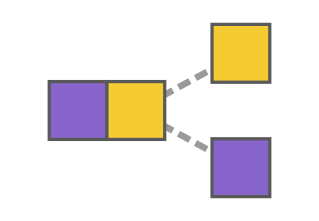
\includegraphics[width=\fwidth]{fig/term-subfun.png} & %
		Subfunctionalization & $x_p^kx_p^j\sum_{n\neq m}x_n^k(1-x_n^j)(1-x_m^k)x_m^j$  \\
	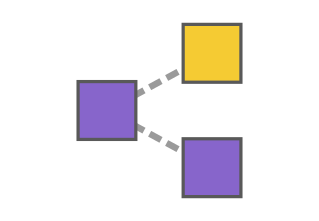
\includegraphics[width=\fwidth]{fig/term-neofun.png} & %
		Neofunctionalization & $x_p^k(1 - x_p^j)\sum_{n\neq m}x_n^k(1-x_n^j)(1-x_m^k)x_m^j$ \\
	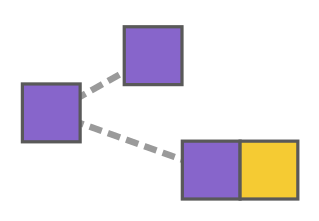
\includegraphics[width=\fwidth]{fig/term-longest.png} & %
		Longest branch gains & $(1-x_p^k)\isone{x_m^k : m=\text{argmax}_n\text{blength}_n}$ \\
	\bottomrule
	\end{tabular}
	\caption{\textit{Example of sufficient statistics for evolutionary transitions}. $x_n^i \in \{0,1\}$, equal to 1 if the function $i$ is present in gene $n$. The $p$ subscript denotes parent gene.}
	\end{table}
 \normalsize
 \end{minipage}
 
\end{frame}

\begin{frame}{GEESE: \textbf{GE}ne functional \textbf{E}volution using \textbf{S}ufici\textbf{E}ncy}

I implemented what I just described in a C++ library with a companion R package called geese. The question is: How much do we earn by using these motifs?\\\bigskip
\pause
\begin{itemize}[<+->]
    \item Using 37 phylogenetic trees featuring 401 go annotations.
    \item \textbf{aphylo}: Fitted a \textit{simple gain/loss} of function model.
    \item \textbf{GEESE}: Fitted an evolutionary model controlling for \textit{functional preservation} (\textit{i.e.}, only one offspring changes)
    \item Fitted both of them using MCMC.
    \item Used LOO cross-validation to compute aggregated AUCs and MAE.
\end{itemize}
\end{frame}

\begin{frame}{GEESE for predicting gene function (cont.)}

How much can we gain from a joint dist. model?
    
\begin{figure}
\centering
    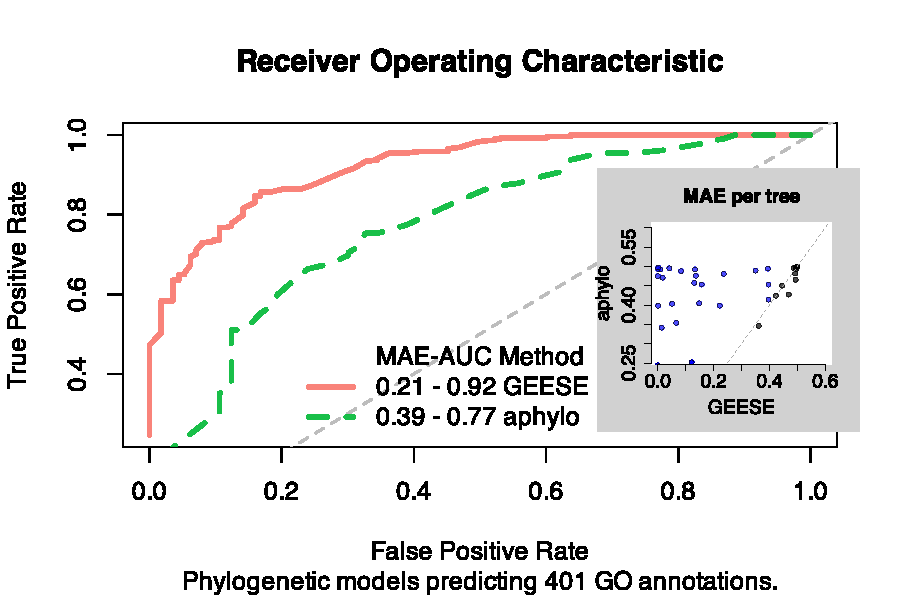
\includegraphics[width = .7\linewidth]{fig/mcmc-analysis-unif-prior-curated-auc-and-mae.pdf}
    % \caption{Caption}
    \label{fig:auc-geese-vs-aphylo}
\end{figure}

Just controlling for preservation (having only one duplicate changing) significantly improves our predictions.
    
\end{frame}

%%%%%%%%%%%%%%%%%%%%%%%%%%%%%%%%%%%%%%%%%%%%%%%%%%%%%%%%%%%%%%%%%%
%%%%%%%%%%%%%%%%%%%%%%%%%%%%%%%%%%%%%%%%%%%%%%%%%%%%%%%%%%%%%%%%%%
\section{Mechanistic Machine Learning}\toc{}

\begin{frame}{Mechanistic Machine Learning: State-of-the-art}

	% \begin{itemize}
		% \item
  After all the data pouring, attention to causal inference and mechanistic models is coming back\autocite{bakerMechanisticModelsMachine2018, pearlSevenToolsCausal2019}
	% 	\item Applications in Physics, Chemistry, Biomedical Imaging, and Biology\autocite{willardIntegratingScientificKnowledge2022a, jornerMachineLearningMeets2021, gawIntegrationMachineLearning2019, altaweraqiImprovedPredictionGene2022} show the benefits of combining the two approaches.
	% \end{itemize}

\begin{center}
	\byside{.4}{Mechanistic Models}{
		\begin{itemize}
			\item Inference-driven (causality).
			\item Great for small datasets.
			\item Knowledge beyond the observed data.
		\end{itemize}
	}
	\byside{.4}{Machine Learning Models}{
		\begin{itemize}
			\item Data-driven (prediction).
			\item Great for big data.
			\item Finds hidden knowledge in observed data.
		\end{itemize}
	}
\end{center}

\end{frame}

\begin{frame}{Mechanistic Machine Learning: State-of-the-art (cont)}

Ways in which it's been applied:

\begin{itemize}
    \item<2-> Adjusting errors in mechanistic-based prediction models (like ABMs).\autocite{compagniHybridNeuralNetworkSEIR2022}
    \item<3-> Incorporating mechanistically inferred data as additional -omics layer.\autocite{zampieriMachineDeepLearning2019}
    \item<4-> Using pathway-networks to add ``external knowledge'' as features.\autocite{altaweraqiImprovedPredictionGene2022}
    \item<5-> Creating a loss-function with a mechanistic penalty for modeling tumor cell-density\autocite{gawIntegrationMachineLearning2019}
    \item<6-> and more...\autocite{jornerMachineLearningMeets2021, willardIntegratingScientificKnowledge2022a, jiaPhysicsGuidedMachineLearning2021, vonruedenInformedMachineLearning2023}
\end{itemize}

\vfill
\uncover<7->{
\footnotesize\alert{Important}: Mechanistic Machine Learning \textbf{is not} domain-knowledge aided feature engineering. You need a whole other model to complement the ML algorithm.
}

\uncover<8->{\alert{Important 2:} This isn't just ML-ensemble, you need to have an ML and a Mech model.\normalsize}
    
\end{frame}

\begin{frame}{Three strategies}
	
	\begin{itemize}
	\item[a.]<2-> \textbf{ML Correction}: Use machine learning to learn the errors of a mechanistic model.
	\item[b.]<3-> \textbf{Mechanistic Feature}: Add mechanistic predictions as a feature of a machine learning model.
	\item[c.]<4-> \textbf{Mechanistic Penalty}: Add constraints to the ML algorithm based on a mechanistic model.
	\end{itemize}

	\begin{figure}
	\centering
	\includegraphics[width=.3\linewidth]{fig/DALL·E 2022-12-07 21.41.30.png}
	\caption{``A van Gogh-style painting of an android holding a large biology book in one hand and a computer in another, examining an evolutionary tree that, instead of leaves, have genes.''--DALL-E's interpretation of my description \hyperlink{https://labs.openai.com/s/s0GoDQ64OMRfMr1y6uRXtmo9}{(link)}}
\end{figure}
\end{frame}

\begin{frame}{Three strategies}
	\framesubtitle{a. ML Correction}
	\begin{minipage}[b]{.4\linewidth}
		\begin{enumerate}[<+->]
			\item Fit the mechanistic model using GEESE
			\item Generate the mechanistic-based predictions, $\AnnPred^{GEESE}$, 
			\item fit an ML model $f(\Features, \Omega)$ to predict $\varepsilon \equiv (\Ann - \AnnPred^{GEESE})$, \item generate the predictions of $\hat\varepsilon$, and 
			\item Compute the Mechanistic-ML predictions as $\AnnPred^{MML1} \equiv \AnnPred^{GEESE} + \hat\varepsilon$
		\end{enumerate}
	\end{minipage}\hfill%
	\begin{minipage}[b]{.55\linewidth}
	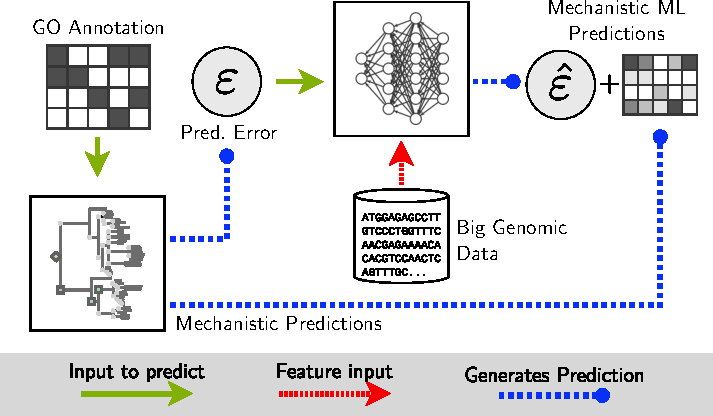
\includegraphics[width=1\linewidth]{fig/mech-ml-model-a.pdf}
	\end{minipage}
\end{frame}

\begin{frame}{Three strategies}
	\framesubtitle{b. Mechanistic Feature}
	\begin{minipage}[b]{.4\linewidth}
		\begin{enumerate}[<+->]
		\item Fit the mechanistic model using GEESE, 
		\item generate the mechanistic-based predictions, $\AnnPred^{GEESE}$, 
		\item fit an ML model that uses the mechanistic predictions as features, $f(\Features, \Omega, \AnnPred^{GEESE})$, and 
		\item Compute the Mechanistic-ML predictions as $\AnnPred^{MML2} \equiv f(\Features, \Omega, \AnnPred^{GEESE})$
		\end{enumerate}
	\end{minipage}\hfill
	\begin{minipage}[b]{.55\linewidth}
		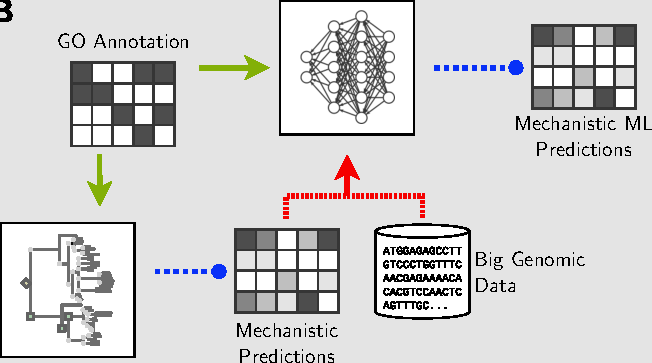
\includegraphics[width=1\linewidth]{fig/mech-ml-model-b.pdf}
	\end{minipage}
\end{frame}

\begin{frame}{Three strategies}
	\framesubtitle{c. Mechanistic Penalty}
	\begin{minipage}[b]{.4\linewidth}
		\begin{enumerate}[<+->]
		\item Fit the mechanistic model using GEESE and store the parameter estimates $\hat\theta$, 
		\item minimize the following loss function: 
		$$
		L(\annObs, \Features, \Omega) - \loglik{f(\annObs, \Features, \Omega)}_{GEESE},$$
		\noindent where $\loglik{\cdot}$ is the likelihood function under GEESE.
		\end{enumerate}
	\end{minipage}\hfill%
	\begin{minipage}[b]{.55\linewidth}
		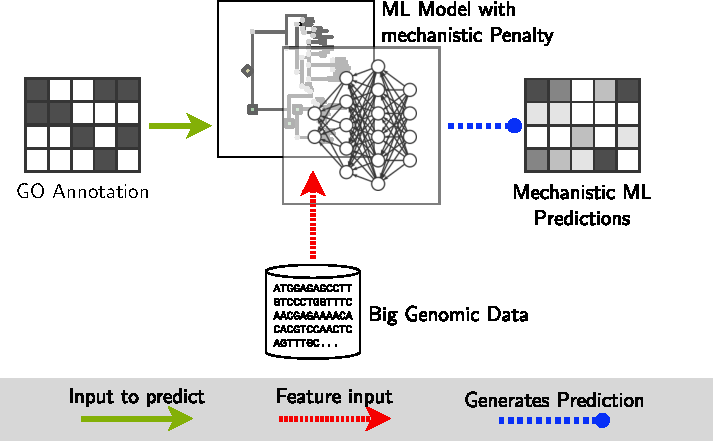
\includegraphics[width=1\linewidth]{fig/mech-ml-model-c.pdf}
	\end{minipage}
\end{frame}

%%%%%%%%%%%%%%%%%%%%%%%%%%%%%%%%%%%%%%%%%%%%%%%%%%%%%%%%%%%%%%%%%%
%%%%%%%%%%%%%%%%%%%%%%%%%%%%%%%%%%%%%%%%%%%%%%%%%%%%%%%%%%%%%%%%%%
\section{Proof of Concept}\toc{}
%%%%%%%%%%%%%%%%%%%%%%%%%%%%%%%%%%%%%%%%%%%%%%%%%%%%%%%%%%%%%%%%%%
%%%%%%%%%%%%%%%%%%%%%%%%%%%%%%%%%%%%%%%%%%%%%%%%%%%%%%%%%%%%%%%%%%

\begin{frame}{Beyond GO and Trees... Bgee}


The 
\includegraphics[width=.1\linewidth]{fig/bgee_logo.png} project ``is a \textbf{database} for retrieval and \textbf{comparison of gene expression} patterns \textbf{across multiple animal species}. It provides an intuitive answer to the question `where is a gene expressed?'[.]'' -- \textcite{bastianBgeeSuiteIntegrated2021}

\vfill

\begin{itemize}
    \item Raw expression annotations.
    \item Standardized expression scores (so can compare across species/tissues).
    \item And also yes/no expression annotations based on the standardized scores.
\end{itemize}

\vfill

\pause Divergence across species in gene expression levels has been linked to evolutionary events\autocite{nabholzHighLevelsGene2013, hodgins-davisEvolvingGeneExpression2009}, \textit{i.e.}, expression levels clustered phylogenies.\\\bigskip
\end{frame}

%%%%%%%%%%%%%%%%%%%%%%%%%%%%%%%%%%%%%%%%%%%%%%%%%%%%%%%%%%%%%%%%%%
%%%%%%%%%%%%%%%%%%%%%%%%%%%%%%%%%%%%%%%%%%%%%%%%%%%%%%%%%%%%%%%%%%

\begin{frame}[t]{What went into the blender}
\small\vspace{-1cm}
\begin{center}
    \uncover<2->{\byside{.45}{Data Feats}{
        \begin{itemize}
            \item Bgee 15 dataset: approx 7 billion annotations for 1.5 million genes.
            \item Our dataset: 1,484 predictions for 1,318 genes.
            \item Search by Gene name: 9,923,427 Bgee annotations.
        \end{itemize}
    }}
    \uncover<3->{\byside{.45}{Final model}{
    \begin{itemize}
        \item 10 GO terms (in a full-Markov model, this is $2^{3\times 10}\sim$1 billion params).
        \item 278 annotations for 256 genes.
        \item 10 GEESE predictions for each gene.
        \item 46 Bgee score for gene expression computed as \textbf{\textit{mean expression score by gene-genus}}
    \end{itemize}
    }}
\end{center}

\vfill
\raggedright
\scriptsize \uncover<4->{\textbf{GO terms}: GO:0004672, GO:0004713, GO:0004867, GO:0005730, GO:0005829, GO:0005886, GO:0006468, GO:0009408, GO:0015020, GO:0060070

\textbf{Genus}: Anguilla, Anolis, Astatotilapia, Astyanax, Bos, Branchiostoma, Caenorhabditis, Callithrix, Canis, Capra, Cavia, Cercocebus, Chlorocebus, Danio, Drosophila, Equus, Esox, Felis, Gadus, Gallus, Gasterosteus, Gorilla, Heterocephalus, Homo, Latimeria, Lepisosteus, Macaca, Manis, Meleagris, Microcebus, Monodelphis, Mus, Neolamprologus, Nothobranchius, Ornithorhynchus, Oryctolagus, Oryzias, Ovis, Pan, Papio, Poecilia, Rattus, Salmo, Scophthalmus, Sus, Xenopus}
\normalsize
\end{frame}

\begin{frame}{Mechanistic ML}

We are comparing three models:

\begin{center}
    \uncover<1->{\byside{.3}{GEESE}{Phylogenetic based predictions (evolution of gene function)}}
    \uncover<2->{\byside{.3}{Bgee}{Linear Prob. model using expression as predictors.}}
    \uncover<3->{\byside{.3}{GEESE + Bgee}{Linear Prob. model using expression as predictors \textbf{and} predictions made by GEESE.}}
\end{center}
    
\end{frame}

\begin{frame}{Mechanistic ML (prelim res.)}
    \begin{figure}
        \centering
        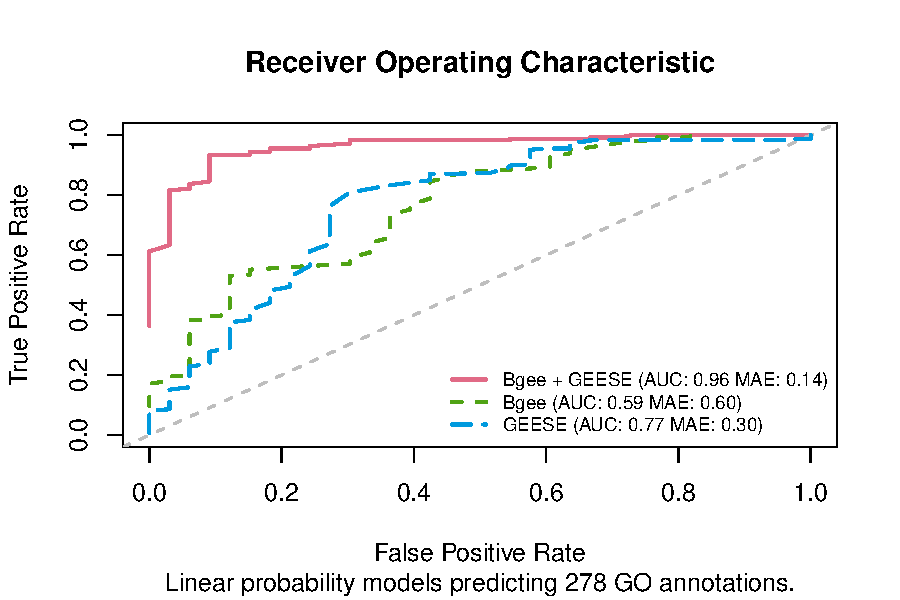
\includegraphics[width = .7\linewidth]{fig/logit-aucs-ols-geese.pdf}
        % \caption{Prelimi results 1}
        \label{fig:auc-geese-plus-bgee}
    \end{figure}
\vfill
\small Both AUC and MAE were computed only using predictions for which we knew the true value.\normalsize
\end{frame}


%%%%%%%%%%%%%%%%%%%%%%%%%%%%%%%%%%%%%%%%%%%%%%%%%%%%%%%%%%%%%%%%%%
%%%%%%%%%%%%%%%%%%%%%%%%%%%%%%%%%%%%%%%%%%%%%%%%%%%%%%%%%%%%%%%%%%

\begin{frame}{}

    \footnotesize This talk has been submitted as an R01 to the National Human Genome Research Institute [NHGRI]\normalsize
    
    \begin{figure}
        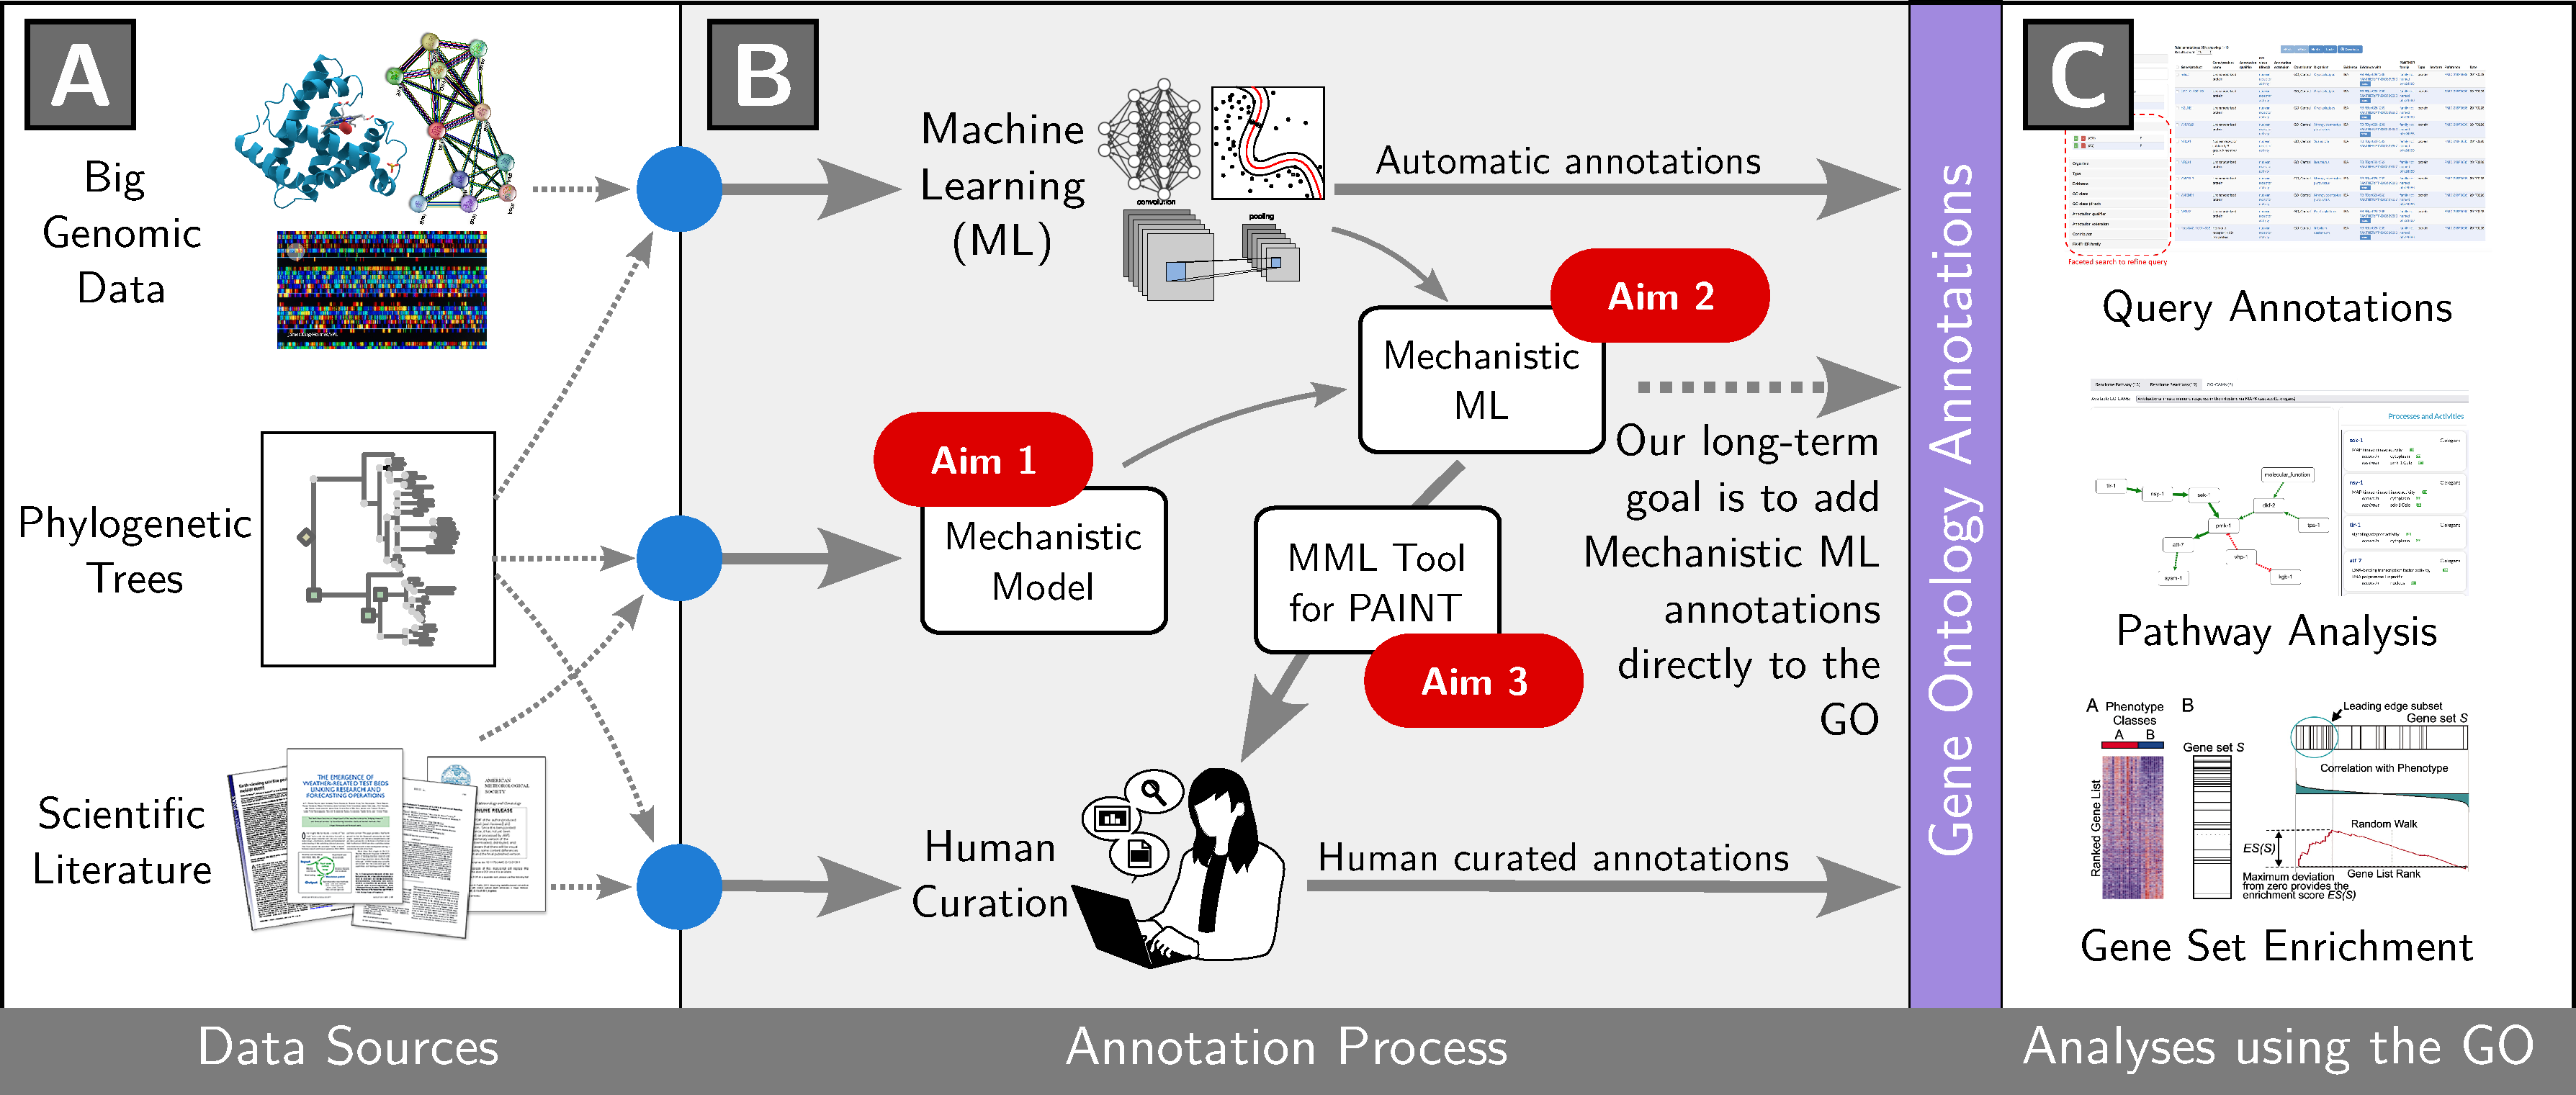
\includegraphics[width=.95\linewidth]{fig/whole-game.pdf}
        \caption{Building a Novel Prediction Framework Leveraging Biological Insights to Boost Machine Learning Algorithms for Annotating Gene Function}
    \end{figure}
    
\end{frame}

\begin{frame}{Discussion}
\uncover<2->{\byside{.32}{\normalsize Gene function}{\small\begin{itemize}
        \item We are racing to discover what genes do.
        \item Experimental assessment is expensive (money and time,) $\to$ automatic annotations.
        \item Many ways to do it (seq. homology, evolutionary theory, ML, etc.)
        \item The best methods use ML (pattern discovery)... but none (AFAIK) are based on bio. theory.
\end{itemize}}}
\uncover<3->{\byside{.32}{\normalsize Evol. Model}{\small\begin{itemize}
    \item We proposed an Evolutionary model of Gene Function.
    \item This new model, GEESE, uses sufficiency to reduce ``Markov complexity.''
    \item We showed it really helps.
\end{itemize}}}
\uncover<4->{\byside{.32}{\normalsize Mechanistic ML}{\small
\begin{itemize}
    \item Mechanistic Machine Learning (mixing theory-based models with ML) promises improved predictions.
    \item I showed an application using gene expression (Bgee).
    \item Adding our mechanistic predictions (based on GEESE) boosted quality
\end{itemize}
}}

\end{frame}

%\begin{frame}{Discussion (cont.)}
%    \begin{itemize}[<+->]
%        \item This is the core of an R01 first submitted in Feb 2022.
%        \item The original version did not feature any ML, just the mechanistic part.
%        \item Two important critiques: ``Not leveraging large genomic data'' and ``Not using Neural Networks''
%        \item We believe we are addressing both using gene expression data (Bgee) and Mechanistic ML.
%        \item ...your thoughts?
%    \end{itemize}
%\end{frame}

\begin{frame}{}
\begin{center}
    \Large Thank you!
\end{center}
\maketitle
\end{frame}

\appendix

\begin{frame}[allowframebreaks]{References}
    \printbibliography
\end{frame}

\begin{frame}[label=aphylo-current]
	\frametitle{Phylogenetics Modeling Strategies}
	
	\begin{minipage}[m]{.3\linewidth}
		
		\begin{figure}
			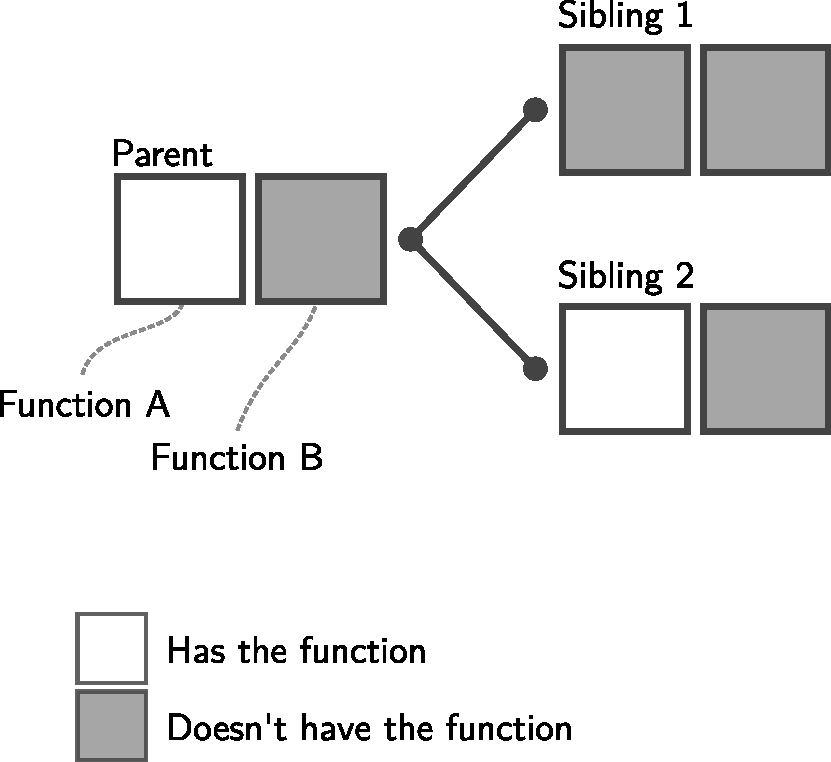
\includegraphics[width=.9\linewidth]{phylo-model-overview-legend.pdf}
		\end{figure}
		
% 		\uncover<5->{\large SNA could help us with\\\alert{\textbf{Exponential\\Random~Graph Models}}}
	\end{minipage}\hfill
	\begin{minipage}[m]{.69\linewidth}
		\mode<beamer>{
			\begin{figure}
				\phantom{\includegraphics<1>[width=.9\linewidth]{phylo-model-overview-1.pdf}}%
				\includegraphics<2>[width=.9\linewidth]{phylo-model-overview-1.pdf}%
				\includegraphics<3>[width=.9\linewidth]{phylo-model-overview-2.pdf}%
				\includegraphics<4>[width=.9\linewidth]{phylo-model-overview.pdf}
			\end{figure}
		}
		
		\mode<handout>{
			\begin{figure}
				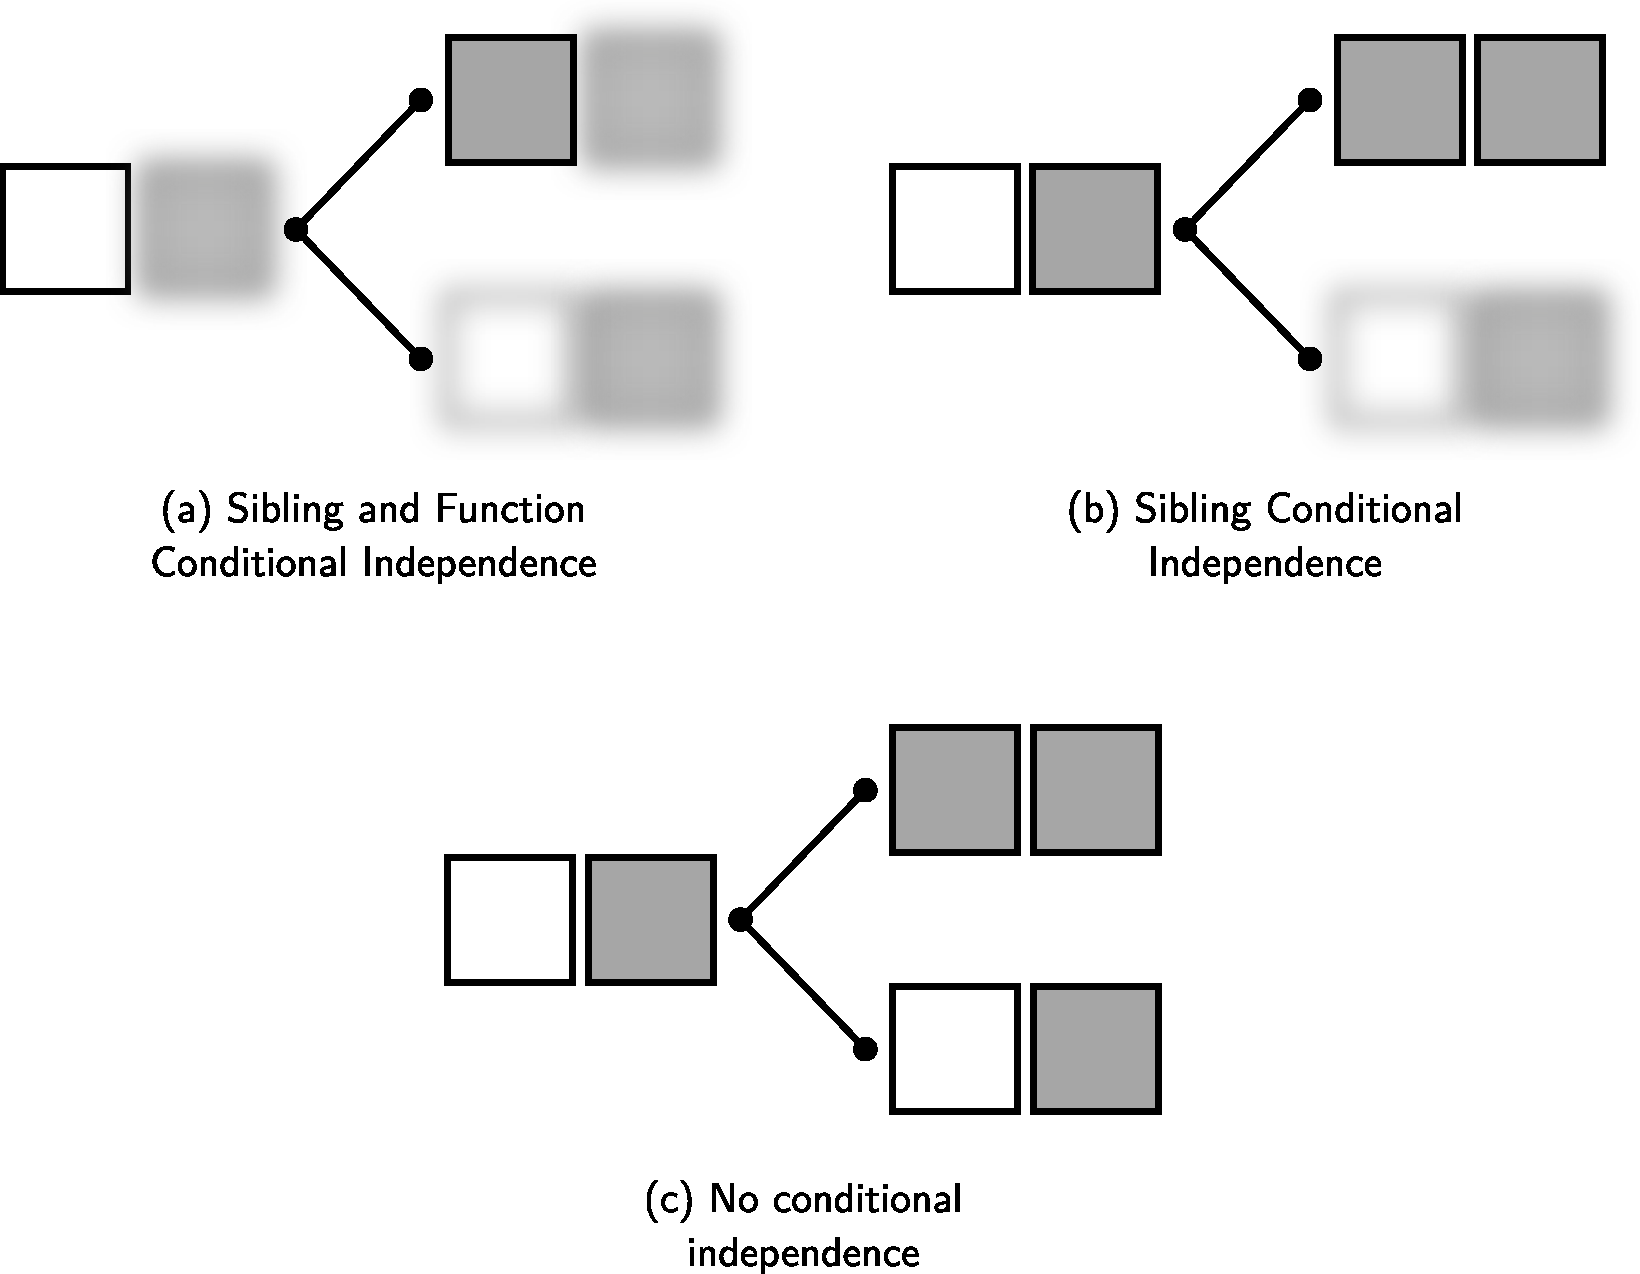
\includegraphics[width=.9\linewidth]{phylo-model-overview.pdf}
			\end{figure}
		}
	\end{minipage}
	
\end{frame}

% ------------------------------------------------------------------------------
\begin{frame}[c]{Evolution of Gene function (multiple functions)}
	
	If we wanted to build a model with 3 functions, we would need to estimate...\\\bigskip
	\begin{minipage}[t]{.40\linewidth}
		\centering
		\shadowbox{Full Markov Transition Matrix}\\\bigskip
		\uncover<1->{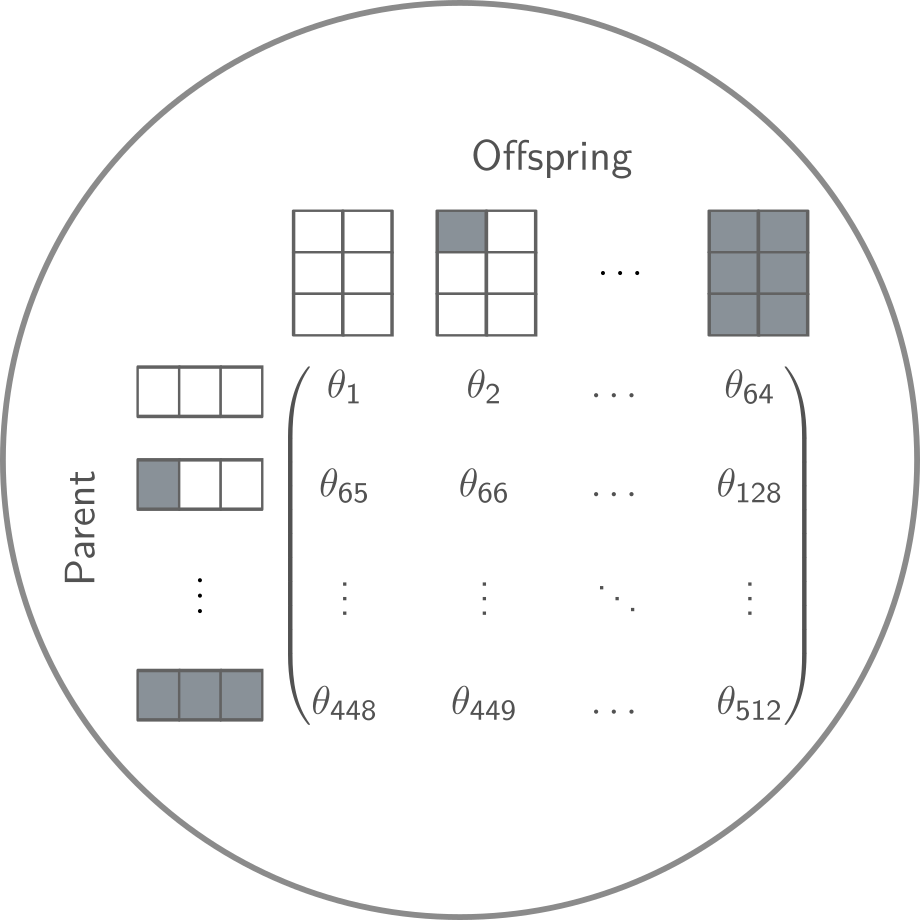
\includegraphics[width=.8\linewidth]{aphylo-ergm-eq1.png} \\
			\vfill 
		}
	\end{minipage}\hfill
	\uncover<2->{\begin{minipage}[t]{.50\linewidth}
	    \vfill
	    \begin{itemize}
	        \item<2-> 512 parameters
	        \item<3-> Finding this many parameters is not easy.
	        \item<4-> Even if you can, interpretation is awkward.
	    \end{itemize}
	\end{minipage}}
	\vfill
\hfill\uncover<5->{Social Network Analysis may help us...}
\end{frame}



% -------------------------------------------------------------------------------
\begin{frame}[t]
	\frametitle{Exponential Random Graph Models (ERGMs)}
	\begin{center}
    \byside{.45}{Social Network}{%
	    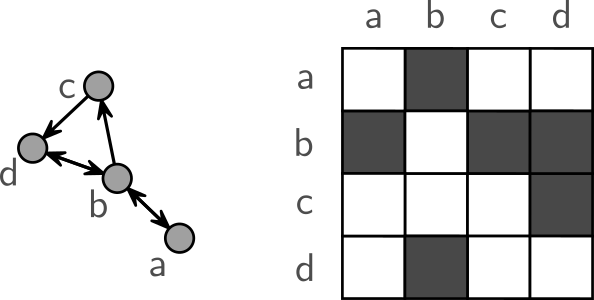
\includegraphics[width=1\linewidth]{fig/adjmat-network.png}
	} \hfill %
	\begin{minipage}[t]{.5\linewidth}
	    \bigskip
	    \begin{itemize}
	    \item<2-> Not about individual ties.
	    \item<3-> Statistical inference on \textit{motifs} (triangles, dyads, homophily, etc.)
            \item<4-> Literature about ERGMs is vast, a.k.a. a low-hanging fruit.
	    \end{itemize}
	    \bigskip
	    \uncover<5->{Ultimately... \\
	    \Large
	    \textbf{ERGM} $\equiv$ \textbf{Modeling binary arrays}
	    \normalsize}
	    
	\end{minipage}
 \end{center}
	
\end{frame}

% -------------------------------------------------------------------------------
\begin{frame}[t]
	\frametitle{Exponential Random Graph Models (ERGMs)}
	\begin{center}
	\byside{.45}{Social Network}{%
	    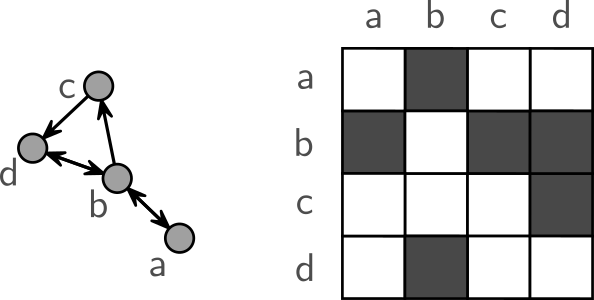
\includegraphics[width=1\linewidth]{fig/adjmat-network.png}
	} \hfill %
	\byside{.45}{Evolutionary Event}{%
	    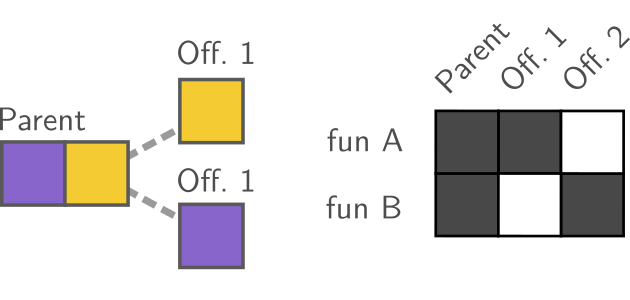
\includegraphics[width=1\linewidth]{fig/adjmat-aphylo.png}
	}
        \end{center}
	\vfill
	Social Networks are usually represented as \textbf{adjacency matrices}, and so can evolutionary events!
	
\end{frame}

%-------------------------------------------------------------------------------
\begin{frame}[c]
\frametitle{Tree likelihoods: Felsenstein's Pruning algorithm}
\begin{center}
    \mode<beamer>{%
    \includegraphics<1>[width=.6\linewidth]{aphylo-equation1.pdf}%
    \includegraphics<2>[width=.6\linewidth]{aphylo-equation.pdf}
    }%
    \mode<handout>{%
    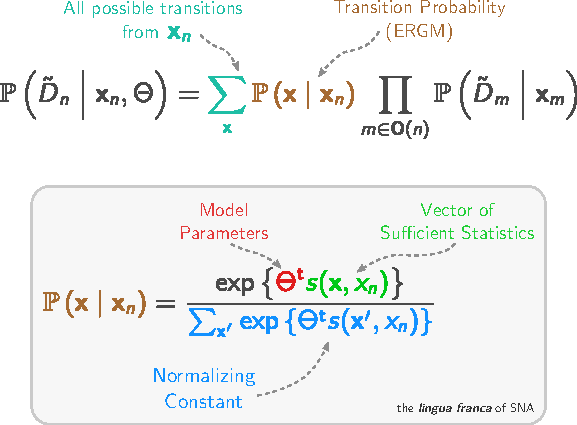
\includegraphics[width=.6\linewidth]{aphylo-equation.pdf}
    }
\end{center}
\vfill\hfill\uncover<2->{... I implemented this (and more) on \textbf{barry}}
\end{frame}

\begin{frame}{Some computational features of \textbf{barry}}
\begin{figure}
    \centering
    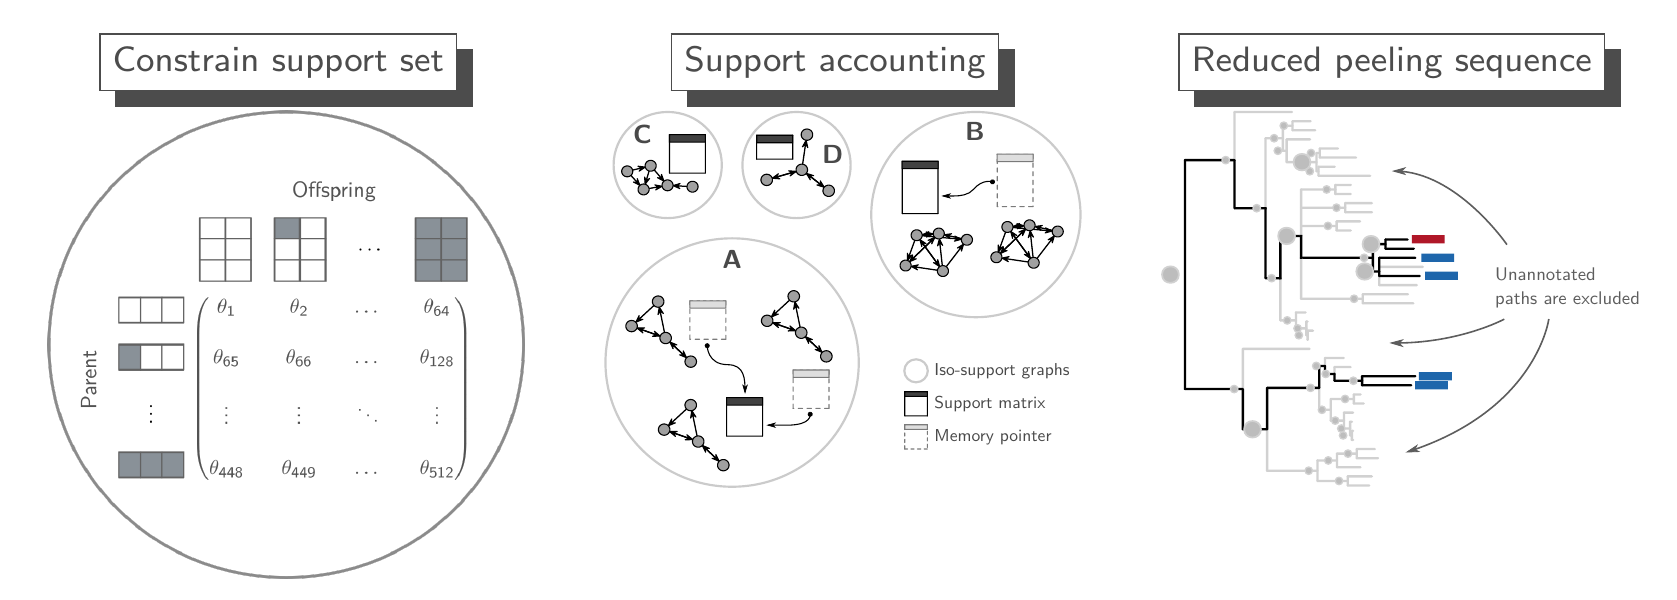
\includegraphics[width=1\textwidth]{fig/barry-computing.png}
    \label{fig:barry}
\end{figure}
\end{frame}

\end{document}